% =====================================================================
%  Neuro-Symbolic Causal Inference — Phase 2 (Deep Learning) Report
%  Compile:  pdflatex Phase2_Report.tex (twice), tectonic, or Overleaf.
%  Figures live in ./figures (Phase 1: tools/make_report_figures.py; fig2_*: the Phase 2 notebook).
% =====================================================================
\documentclass[12pt,a4paper]{article}

% ---------------------------------------------------------------- edit me
\newcommand{\MemberA}{Krishnadevan Manju Liby}
\newcommand{\MemberB}{Hemanth Tenneti}
\newcommand{\MemberC}{Arina Ali}
\newcommand{\MemberD}{Manan Bansal}
\newcommand{\MemberE}{Aaloke Eppalapalli}
\newcommand{\Institution}{Newton School of Technology, Rishihood University}
\newcommand{\Course}{CSAI Student Project --- Applied Machine Learning \& Deep Learning}
\newcommand{\RepoURL}{https://github.com/HemanthTenneti/AML-DL-Project-2026}
\newcommand{\ReportDate}{November 2026}

% ---------------------------------------------------------------- packages
\usepackage[T1]{fontenc}
\usepackage{lmodern}
\usepackage{amsmath,amssymb}
\usepackage[a4paper,margin=2.5cm,headheight=15pt]{geometry}
\usepackage[table]{xcolor}
\usepackage{graphicx,booktabs,tabularx,array,enumitem,microtype,longtable}
\usepackage[nobottomtitles*]{titlesec}
\usepackage{fancyhdr,caption,subcaption,listings}
\renewcommand{\bottomtitlespace}{0.15\textheight}
\usepackage{tikz}
\usetikzlibrary{positioning,arrows.meta,calc,shapes.geometric,fit,backgrounds}
\usepackage{hyperref}
\usepackage[nameinlink,capitalise]{cleveref}

% ---------------------------------------------------------------- colours
\definecolor{navy}{HTML}{1F4E79}     % title, section headings
\definecolor{accent}{HTML}{4A86C5}   % subsection headings, links
\definecolor{rowtint}{HTML}{E8EEF7}  % alternate table rows
\colorlet{slate}{black!55}
% diagram colours (all three pipeline layers share the report's navy)
\colorlet{neural}{navy}\colorlet{symbolic}{navy}\colorlet{causal}{navy}
\colorlet{neuralT}{rowtint}\colorlet{symbolicT}{rowtint}\colorlet{causalT}{rowtint}
\colorlet{ink}{black}

\hypersetup{colorlinks=true,linkcolor=accent,citecolor=accent,urlcolor=accent,
  pdftitle={Neuro-Symbolic Causal Inference -- Phase 2 Report},pdfauthor={Team Project 1}}

% ---------------------------------------------------------------- headings
\titleformat{\section}{\Large\bfseries\color{navy}}{\thesection.}{0.5em}{}[\vspace{2pt}{\color{navy}\titlerule[0.6pt]}]
\titleformat{\subsection}{\large\bfseries\color{accent}}{\thesubsection.}{0.5em}{}
\titleformat{\subsubsection}{\normalsize\bfseries}{\thesubsubsection.}{0.5em}{}
\titlespacing*{\section}{0pt}{1.4em}{0.8em}
\titlespacing*{\subsection}{0pt}{1.1em}{0.5em}
\titlespacing*{\subsubsection}{0pt}{1.0em}{0.4em}

% ---------------------------------------------------------------- header/footer
\pagestyle{fancy}\fancyhf{}
\fancyhead[L]{\small\bfseries\color{navy}Neuro-Symbolic Causal Inference}
\fancyhead[R]{\small\color{accent}Phase 2 Report}
\fancyfoot[C]{\thepage}
\renewcommand{\headrulewidth}{0.4pt}
\renewcommand{\footrulewidth}{0.4pt}

% ---------------------------------------------------------------- captions, lists, tables
\captionsetup{labelsep=colon,margin=0.5em}
\setlist{leftmargin=1.4em,itemsep=0.25em,topsep=0.4em}
\renewcommand{\arraystretch}{1.25}
\setlength{\emergencystretch}{2em} % let long code names wrap the line instead of running into the margin
\newcommand{\thead}[1]{\textbf{#1}}
\makeatletter % float pages: stack floats from the top instead of centring them
\setlength{\@fptop}{0pt}\setlength{\@fpsep}{1.5em}\setlength{\@fpbot}{0pt plus 1fil}
\makeatother

% ---------------------------------------------------------------- plain environments
\newenvironment{theorybox}[1]{\subsubsection*{#1}}{}
\newenvironment{keybox}{\par\medskip\noindent\textbf{Key takeaway.}\ }{\par\medskip}
\newenvironment{examplebox}{\begin{quote}}{\end{quote}}
\newcommand{\code}[1]{\texttt{#1}}
\newcommand{\doop}{\mathrm{do}}

\lstset{basicstyle=\ttfamily\footnotesize,keywordstyle=\bfseries,commentstyle=\itshape,
  frame=none,xleftmargin=0pt,aboveskip=8pt,belowskip=8pt,columns=fullflexible,keepspaces=true,
  showstringspaces=false,language=Python}


% =====================================================================
\begin{document}

% ---------------------------------------------------------------- title page
\begin{titlepage}
\centering
\vspace*{2.2cm}
{\color{navy}\rule{\linewidth}{0.8pt}}\par\vspace{1.0cm}
{\Huge\bfseries\color{navy} Neuro-Symbolic Causal Inference\par}
\vspace{0.4cm}
{\Large\bfseries\color{navy} via Language-Model Knowledge Extraction\\[0.15em] and Bayesian Networks\par}
\vspace{0.9cm}
{\color{navy}\rule{\linewidth}{0.8pt}}\par\vspace{1.1cm}
{\large\bfseries\color{accent} Project 1 --- Phase 2: Deep Learning Evaluation\par}
\vspace{0.6cm}
{\large \Course\par}
\vspace{1.2cm}
\begin{tabular}{@{}>{\bfseries}l l@{}}
Dataset     & Corr2Cause (Jin et al., ICLR 2024), corrected labels \\
Model       & DistilBERT (\texttt{distilbert-base-cased}, 66\,M parameters) \\
Framework   & PyTorch, Hugging Face Transformers, scikit-learn, NetworkX, pgmpy \\
Institution & \Institution \\
Repository  & \small\url{\RepoURL} \\
\end{tabular}
\par\vspace{1.4cm}
{\color{navy}\rule{0.6\linewidth}{0.6pt}}\par\vspace{0.6cm}
{\large\bfseries Team Members\par}\vspace{0.2cm}
{\large \MemberA\\ \MemberB\\ \MemberC\\ \MemberD\\ \MemberE\par}
\vfill
{\large \ReportDate\par}
\end{titlepage}

% ---------------------------------------------------------------- contents
\setcounter{page}{1}
\setcounter{tocdepth}{2}
\tableofcontents
\newpage

% =====================================================================
\section{Abstract}
Phase~1 built a three-layer pipeline for Corr2Cause~\cite{jin2024corr2cause}: a regex \emph{language layer} reads the
text, a \emph{reasoning layer} (PC algorithm~\cite{spirtes2000} + a depth-4 decision tree) decides which causal claims are
entailed, and a \emph{graph layer} turns accepted claims into a DAG, a Bayesian network and intervention answers. It scored
F1~0.997 on test but \textbf{0.000 on paraphrased hypotheses}, because the regex cannot read new wordings.

Phase~2 brings in DistilBERT~\cite{sanh2019} in two ways. \textbf{2A} fine-tunes it end to end on (hypothesis, premise)
pairs, with and without a variable-renaming augmentation. \textbf{2B}, our hybrid, uses DistilBERT \emph{only} as the
language layer and keeps the Phase~1 reasoning and graph layers unchanged. 2A ties the TF-IDF baseline on test
(F1 0.653 vs 0.655): learning causal discovery from text alone does not work at this scale. Renaming augmentation lifts its
score on renamed variables from 0.377 to 0.592. 2B reads \textbf{100\%} of paraphrased hypotheses correctly and raises
paraphrase F1 from \textbf{0.000 to 0.997}; from paraphrased text it rebuilds all \textbf{73/73} gold cause edges and
answers \textbf{97.5\%} of 242 intervention queries, exactly as Phase~1 does on the original text.

% =====================================================================
\section{Introduction}

Phase~1 ended with one clear failure: when Corr2Cause rewords a hypothesis (``A directly causes B'' becomes
``A directly affects B''), the regex reader returns nothing and the system can only answer ``not valid''. The project
brief asks us to ``fine-tune a compact transformer such as DistilBERT for causal relation extraction'' and to
``feed only reviewed predictions into the graph stage''. Phase~2 does exactly that, and asks one question: \emph{where}
should the transformer go?

\begin{figure}[!htbp]
\centering
\resizebox{\linewidth}{!}{%
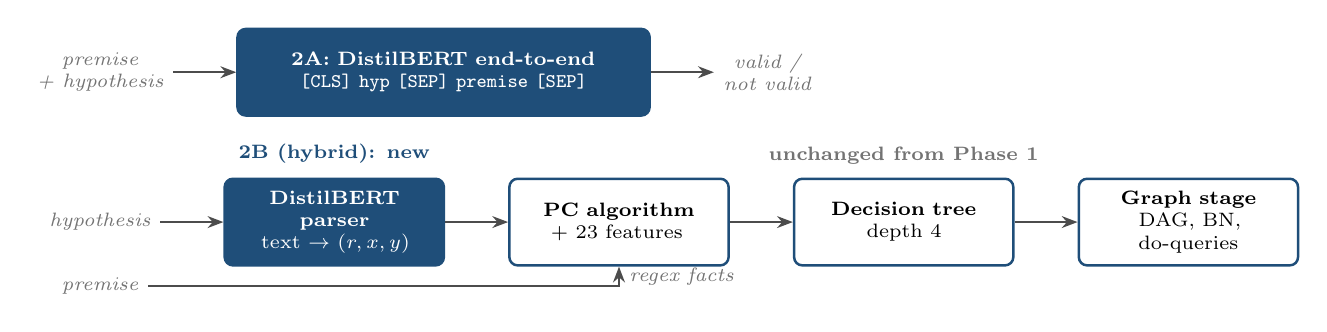
\begin{tikzpicture}[
  stage/.style={draw=navy,fill=white,rounded corners=3pt,line width=0.9pt,minimum height=1.1cm,
                text width=2.55cm,align=center,font=\scriptsize},
  dl/.style={stage,fill=navy,text=white},
  data/.style={font=\scriptsize\itshape,text=slate,align=center},
  flow/.style={-{Stealth[length=2mm]},line width=0.9pt,ink!70},
  node distance=0.8cm]
  % 2A
  \node[data] (a0) {premise\\+ hypothesis};
  \node[dl, right=of a0, text width=5.0cm] (a1) {\textbf{2A: DistilBERT end-to-end}\\\code{[CLS] hyp [SEP] premise [SEP]}};
  \node[data, right=of a1] (a2) {valid /\\not valid};
  \draw[flow] (a0)--(a1); \draw[flow] (a1)--(a2);
  % 2B
  \node[data, below=1.3cm of a0] (b0) {hypothesis};
  \node[dl, right=of b0] (b1) {\textbf{DistilBERT parser}\\text $\rightarrow$ $(r,x,y)$};
  \node[stage, right=of b1] (b2) {\textbf{PC algorithm}\\+ 23 features};
  \node[stage, right=of b2] (b3) {\textbf{Decision tree}\\depth 4};
  \node[stage, right=of b3] (b4) {\textbf{Graph stage}\\DAG, BN, do-queries};
  \node[data, below=0.35cm of b0] (p0) {premise};
  \draw[flow] (b0)--(b1); \draw[flow] (b1)--(b2); \draw[flow] (b2)--(b3); \draw[flow] (b3)--(b4);
  \draw[flow] (p0) -| node[data,pos=0.75,right]{regex facts} (b2);
  \node[font=\scriptsize\bfseries,text=navy,above=0.05cm of b1] {2B (hybrid): new};
  \node[font=\scriptsize\bfseries,text=slate,above=0.05cm of b3] {unchanged from Phase 1};
\end{tikzpicture}}
\caption{The two Phase~2 systems. Filled boxes are DistilBERT. 2A must learn both the language and the causal reasoning
from examples. 2B gives DistilBERT only the language job and keeps the Phase~1 reasoning and graph layers, which are
correct by construction.}
\label{fig:systems}
\end{figure}

\paragraph{Contributions of Phase 2.}
\begin{itemize}
  \item Two DistilBERT systems (\cref{fig:systems}) evaluated on the same splits, metrics and graph code as Phase~1, giving a
        clean $2\times2$ comparison: ML vs DL, text-only vs hybrid (\cref{tab:grid}).
  \item A hybrid (2B) whose transformer parser reads relation \emph{and direction} (6 labels), trained only on
        sentences from a small grammar we wrote, with the official paraphrase wordings provably excluded from training.
  \item A variable-renaming augmentation that removes a known dataset shortcut from the end-to-end model.
  \item Four ablations that each change one part and keep the rest fixed (\cref{sec:ablation}).
  \item A plain, readable PyTorch training loop, 18 new unit tests, and an executed notebook (\cref{sec:repro}).
\end{itemize}

\begin{table}[!htbp]
\centering\small
\caption{The Phase~2 comparison grid. Same splits, same metrics, same graph stage.}
\label{tab:grid}
\begin{tabularx}{\linewidth}{@{}l>{\raggedright}X>{\raggedright\arraybackslash}X@{}}
\toprule
& \thead{Text only (no reasoning layer)} & \thead{Language layer + reasoning layer (hybrid)} \\
\midrule
\textbf{ML (Phase 1)} & TF-IDF + logistic regression & Regex rules + PC + Decision Tree \\
\rowcolor{rowtint}\textbf{DL (Phase 2)} & \textbf{2A}: DistilBERT end-to-end, $\pm$ renaming augmentation &
  \textbf{2B}: DistilBERT parser + PC + Decision Tree \\
\bottomrule
\end{tabularx}
\end{table}

\begin{table}[!htbp]
\centering\small
\caption{Where each Phase~2 evaluation criterion and each requirement of the project brief is addressed.}
\label{tab:rubric}
\begin{tabularx}{\linewidth}{@{}>{\raggedright}p{5.4cm}X@{}}
\toprule
\thead{Criterion / brief requirement} & \thead{Section(s)} \\
\midrule
Deep learning literature review & \cref{sec:lit}, incl.\ where each reference is used (\cref{tab:refuse}) \\
\rowcolor{rowtint} Architecture logic & \cref{sec:arch} \\
Hybrid innovation & \cref{sec:arch2b,sec:data2b} (DistilBERT language layer + symbolic reasoning) \\
\rowcolor{rowtint} Theoretical rigour & \cref{sec:theory} \\
DL dataset \& regularization & \cref{sec:data} \\
\rowcolor{rowtint} Technical validation & \cref{sec:results} (held-out test, renamed and paraphrased sets, held-out verbs) \\
Ablation studies & \cref{sec:ablation} \\
\rowcolor{rowtint} GitHub repository \& code quality & \cref{sec:repro} \\
``Fine-tune a compact transformer such as DistilBERT'' & \cref{sec:arch,sec:data} \\
\rowcolor{rowtint} ``Feed only reviewed predictions into the graph stage'' & \cref{sec:graph} (threshold 0.5, cycle and self-loop rejection) \\
Precision, recall and F1 on a held-out set; edge precision; known intervention queries & \cref{tab:main,tab:graph} \\
\rowcolor{rowtint} ``Visualise a DAG, answer a few documented causal queries'' & \cref{fig:dag,tab:queries} \\
\bottomrule
\end{tabularx}
\end{table}

% =====================================================================
\section{Deep Learning Literature Review}\label{sec:lit}

\subsection{Transformers, BERT and DistilBERT}
The Transformer~\cite{vaswani2017} replaced recurrence with self-attention, letting every token attend to every other token
in one step. BERT~\cite{devlin2019} pre-trains a Transformer encoder with masked-language modelling and showed that
adding one classification layer on the \code{[CLS]} token and fine-tuning the whole network gives strong results on
sentence-pair tasks such as natural language inference. DistilBERT~\cite{sanh2019} compresses BERT by knowledge
distillation~\cite{hinton2015}: a 6-layer student keeps about 97\% of BERT's language-understanding performance with 40\%
fewer parameters and 60\% faster inference. \textbf{We use DistilBERT} because the brief names it, because 66\,M parameters
fit a laptop GPU, and because our language task (short, templated sentences) does not need a larger model.

\subsection{How to fine-tune well}
Fine-tuning a pre-trained model on a small dataset is unstable and overfits easily. Howard and Ruder~\cite{howard2018}
introduced a short warm-up followed by a decaying learning rate; BERT's authors recommend learning rates of
$2\text{--}5\times10^{-5}$ for 2--4 epochs~\cite{devlin2019}, and Sun et al.~\cite{sun2019} found that a small rate
($2\times10^{-5}$) avoids catastrophically forgetting the pre-trained knowledge; Mosbach et al.~\cite{mosbach2021} traced
most fine-tuning failures to optimisation problems and recommend small learning rates with bias-corrected Adam.
AdamW~\cite{loshchilov2019} decouples weight decay from the gradient update, which is the form used for BERT.
Dropout~\cite{srivastava2014} (built into DistilBERT), early stopping on a validation set~\cite{prechelt1998} and
gradient-norm clipping~\cite{pascanu2013} complete the standard recipe. For the class imbalance (21\% valid) we use
inverse-frequency class weights, a standard cost-sensitive fix~\cite{he2009}. \textbf{Every one of these choices is in
our training loop} (\cref{tab:hparams,tab:reg}).

\subsection{Shortcut learning and robustness tests}
Fine-tuned models often succeed for the wrong reasons. In natural language inference, hypothesis-only cues predict the
label~\cite{gururangan2018}, and models adopt shallow heuristics such as word overlap that a targeted test set
exposes~\cite{mccoy2019}; Geirhos et al.~\cite{geirhos2020} call this \emph{shortcut learning}. Corr2Cause's authors fine-tuned
BERT-style models and found exactly this: high in-distribution scores that collapse under paraphrasing and variable
renaming~\cite{jin2024corr2cause}. Behavioural testing with controlled perturbations~\cite{ribeiro2020} is the remedy for
\emph{measuring} it, and training on minimally changed examples whose label is known~\cite{kaushik2020}, a form of data
augmentation~\cite{wei2019}, is a remedy for \emph{reducing} it. \textbf{Our renaming augmentation} (\cref{sec:data2a}) is a
label-preserving perturbation in this spirit, and our refactorization and paraphrase evaluations are behavioural tests.

\subsection{Training a parser on grammar-generated sentences}
When annotated sentences are scarce, semantic parsers can be trained on sentences written by a grammar. Wang, Berant and
Liang~\cite{wang2015} generate canonical utterances from a grammar to build a parser ``overnight'', and Jia and
Liang~\cite{jia2016} show that recombining grammar fragments into new training examples improves generalisation. A caution
comes from Lake and Baroni~\cite{lake2018}: neural models generalise poorly to \emph{unseen combinations} of known parts,
so held-out compositions are the honest test. \textbf{Our 2B parser follows this line}: it learns from a grammar of
verbs $\times$ voice $\times$ modifiers (\cref{sec:data2b}), and we validate on verbs it has never seen.

\subsection{Neuro-symbolic hybrids}
Neuro-symbolic AI pairs learned perception with explicit reasoning~\cite{garcez2023}. The Neuro-Symbolic Concept
Learner~\cite{mao2019} is a well-known example: a neural network parses the input into symbols and a symbolic program
executes on them, which makes the reasoning exact and interpretable. Surveys of language models and causality reach the
same conclusion from the other side: fluent causal language is not causal inference~\cite{kiciman2023}. \textbf{2B is
this design}: DistilBERT parses, the PC algorithm~\cite{spirtes2000,meek1995} and the Bayesian network~\cite{pearl1988,pearl2009}
reason.

\subsection{Where each reference is used}
The Phase~1 review cited the causal-discovery literature but did not show where each paper enters the work.
\Cref{tab:refuse} lists every reference with the idea we take from it and the place in the code and in this report where
it is used.

\begingroup
\footnotesize
\setlength{\tabcolsep}{3pt}
\begin{longtable}{@{}>{\raggedright}p{2.4cm}>{\raggedright}p{6.1cm}>{\raggedright\arraybackslash}p{5.8cm}@{}}
\caption{Every reference, what we use from it, and where.}\label{tab:refuse}\\
\toprule
\thead{Reference} & \thead{What we use} & \thead{Where (code / report)} \\
\midrule
\endfirsthead
\toprule
\thead{Reference} & \thead{What we use} & \thead{Where (code / report)} \\
\midrule
\endhead
\multicolumn{3}{@{}l}{\textit{Data and task}}\\
Jin et al.~\cite{jin2024corr2cause} & Corr2Cause data, robustness sets, the finding that fine-tuned models take shortcuts & \code{data.py}; \cref{sec:data,sec:results} \\
\rowcolor{rowtint} Corrected labels~\cite{corr2causecorrected} & bug-fixed labels used for all scores & \code{data.py}; Phase~1 report \\
\multicolumn{3}{@{}l}{\textit{Causal reasoning (Phase 1, reused unchanged by 2B)}}\\
Spirtes et al.~\cite{spirtes2000} & PC algorithm: skeleton + v-structures from independence facts & \code{causal\_rules.py}; \cref{sec:arch2b} \\
\rowcolor{rowtint} Verma \& Pearl~\cite{verma1990} & Markov equivalence: skeleton + v-structures & \code{causal\_rules.py} (equivalent DAGs) \\
Meek~\cite{meek1995} & orientation rules R1--R3 & \code{causal\_rules.py} \\
\rowcolor{rowtint} Pearl~\cite{pearl1988,pearl2009} & Bayesian networks, do-operator, truncated factorisation & \code{graph\_stage.py}; \cref{sec:graph} \\
Ankan \& Panda~\cite{ankan2015} & pgmpy: network, \code{CausalInference} & \code{graph\_stage.py} \\
\rowcolor{rowtint} Khoo et al.~\cite{khoo2000}, Girju~\cite{girju2003} & pattern-based causal extraction & \code{parsing.py} (Phase~1 regex, the 2B baseline) \\
\multicolumn{3}{@{}l}{\textit{Deep learning model}}\\
Vaswani et al.~\cite{vaswani2017} & self-attention encoder & DistilBERT itself; \cref{sec:theory} (T5) \\
\rowcolor{rowtint} Devlin et al.~\cite{devlin2019} & \code{[CLS]} classification head, sentence-pair input & \code{dl\_end2end.py} (2A input format); \code{dl\_parser.py} \\
Sanh et al.~\cite{sanh2019}, Hinton et al.~\cite{hinton2015} & distilled 6-layer model, 66\,M parameters & \code{dl\_common.py} (\code{MODEL\_NAME}) \\
\rowcolor{rowtint} Wolf et al.~\cite{wolf2020}, Paszke et al.~\cite{paszke2019} & Transformers library, PyTorch & \code{dl\_common.py} \\
\multicolumn{3}{@{}l}{\textit{Training and regularization}}\\
Loshchilov \& Hutter~\cite{loshchilov2019} & AdamW, weight decay 0.01 & \code{train\_classifier}; \cref{tab:hparams} \\
\rowcolor{rowtint} Howard \& Ruder~\cite{howard2018} & warm-up then linear decay & \code{get\_linear\_schedule\_with\_warmup}; \cref{tab:reg} \\
Devlin et al.~\cite{devlin2019}, Sun et al.~\cite{sun2019}, Mosbach et al.~\cite{mosbach2021} & learning rates $2\text{--}5\times10^{-5}$, 2--3 epochs, small-rate stability & \code{train\_phase2.py} configs; \cref{tab:hparams} \\
\rowcolor{rowtint} Srivastava et al.~\cite{srivastava2014} & dropout 0.1 & DistilBERT default; \cref{tab:reg} \\
Prechelt~\cite{prechelt1998} & early stopping on a validation score & \code{train\_classifier} (best epoch kept) \\
\rowcolor{rowtint} Pascanu et al.~\cite{pascanu2013} & gradient-norm clipping at 1.0 & \code{train\_classifier} \\
He \& Garcia~\cite{he2009} & inverse-frequency class weights & \code{train\_classifier}; \cref{sec:theory} (T6) \\
\multicolumn{3}{@{}l}{\textit{Robustness, augmentation and training data}}\\
\rowcolor{rowtint} Gururangan et al.~\cite{gururangan2018}, McCoy et al.~\cite{mccoy2019}, Geirhos et al.~\cite{geirhos2020} & shortcut learning; targeted test sets expose it & \cref{sec:data2a,sec:errors} (letter-order shortcut) \\
Ribeiro et al.~\cite{ribeiro2020} & behavioural tests with controlled perturbations & refactorization / paraphrase evaluation, \cref{sec:results} \\
\rowcolor{rowtint} Kaushik et al.~\cite{kaushik2020}, Wei \& Zou~\cite{wei2019} & label-preserving augmentation & \code{rename\_variables}, \code{augment} in \code{dl\_end2end.py} \\
Wang et al.~\cite{wang2015}, Jia \& Liang~\cite{jia2016} & train a parser on grammar-generated sentences & \code{paraphrase\_grammar.py}; \cref{sec:data2b} \\
\rowcolor{rowtint} Lake \& Baroni~\cite{lake2018} & test on unseen compositions & held-out-verb validation in \code{dl\_parser.py} \\
\multicolumn{3}{@{}l}{\textit{Hybrid design}}\\
Garcez \& Lamb~\cite{garcez2023}, Mao et al.~\cite{mao2019} & neural parser + symbolic executor & 2B architecture, \cref{sec:arch2b} \\
\rowcolor{rowtint} K{\i}c{\i}man et al.~\cite{kiciman2023} & language models alone are not causal reasoners & motivation for 2B; \cref{sec:conclusion} \\
\bottomrule
\end{longtable}
\endgroup

% =====================================================================
\section{Architecture}\label{sec:arch}

Both systems use \code{distilbert-base-cased}. It must be \emph{cased}: variables are single capital letters, and an
uncased tokenizer would turn the variable ``A'' into the English word ``a''.
\Cref{fig:distilbert} shows the network. The WordPiece tokenizer turns the text into token IDs. Each ID looks up a learned
768-dimensional word vector, to which a learned position vector (one row per position, up to 512) is added.
Six identical transformer blocks~\cite{vaswani2017} follow, each with multi-head self-attention and a feed-forward
layer, both wrapped in a residual connection and LayerNorm. DistilBERT has no token-type (segment) embeddings, so the two
segments of 2A are told apart only by \code{[SEP]}. The classification head reads the final vector of \code{[CLS]}.
Only the head is new; the rest starts from the pre-trained weights and is fine-tuned.

\begin{figure}[!htbp]
\centering
\resizebox{\linewidth}{!}{%
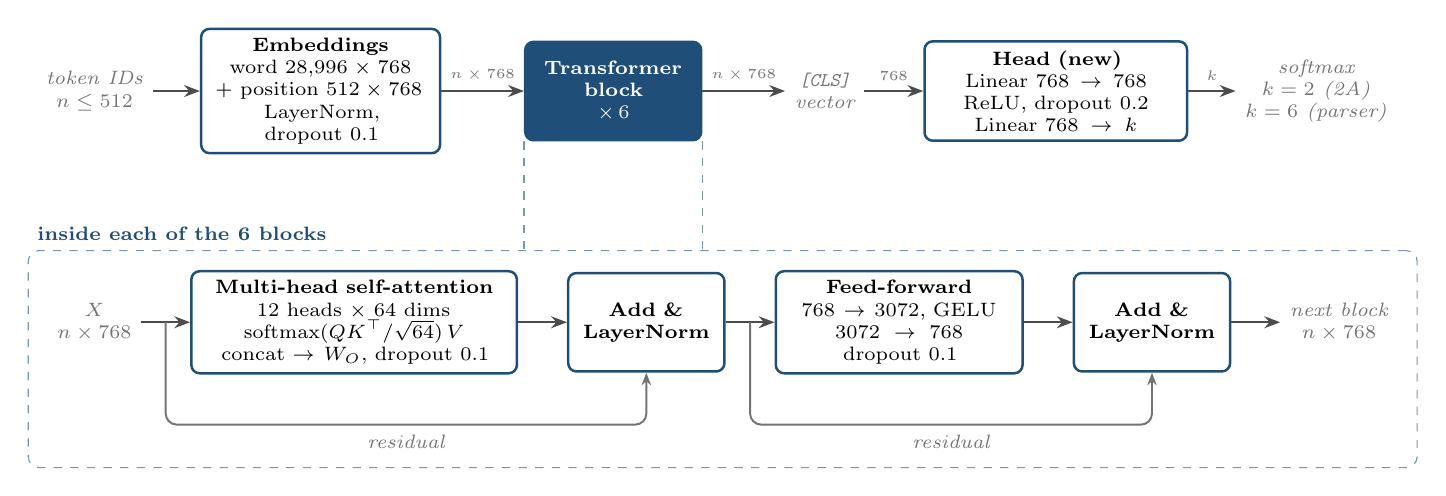
\begin{tikzpicture}[
  stage/.style={draw=navy,fill=white,rounded corners=3pt,line width=0.9pt,minimum height=1.25cm,
                text width=#1,align=center,font=\scriptsize},
  stage/.default=2.5cm,
  dl/.style={stage=#1,fill=navy,text=white},
  dl/.default=2.0cm,
  data/.style={font=\scriptsize\itshape,text=slate,align=center},
  dim/.style={font=\tiny,text=slate,above,midway},
  flow/.style={-{Stealth[length=2mm]},line width=0.9pt,ink!70},
  res/.style={-{Stealth[length=1.6mm]},line width=0.7pt,ink!55,rounded corners=4pt},
  node distance=0.62cm]
  % ---- whole model
  \node[data] (in) {token IDs\\$n\le512$};
  \node[stage=2.8cm, right=0.6cm of in] (emb) {\textbf{Embeddings}\\word $28{,}996\times768$\\+ position $512\times768$\\LayerNorm, dropout 0.1};
  \node[dl, right=1.05cm of emb] (blk) {\textbf{Transformer block}\\$\times\,6$};
  \node[data, right=1.05cm of blk] (cls) {\code{[CLS]}\\vector};
  \node[stage=3.1cm, right=0.75cm of cls] (head) {\textbf{Head (new)}\\Linear $768\to768$\\ReLU, dropout 0.2\\Linear $768\to k$};
  \node[data, right=0.6cm of head] (out) {softmax\\$k=2$ (2A)\\$k=6$ (parser)};
  \draw[flow] (in)--(emb);
  \draw[flow] (emb)--node[dim]{$n\times768$}(blk);
  \draw[flow] (blk)--node[dim]{$n\times768$}(cls);
  \draw[flow] (cls)--node[dim]{768}(head);
  \draw[flow] (head)--node[dim]{$k$}(out);
  % ---- inside one block
  \node[data, below=2.2cm of in] (x) {$X$\\$n\times768$};
  \node[stage=3.9cm, right=of x] (mha) {\textbf{Multi-head self-attention}\\12 heads $\times$ 64 dims\\$\mathrm{softmax}(QK^{\top}/\sqrt{64})\,V$\\concat $\to W_O$, dropout 0.1};
  \node[stage=1.75cm, right=of mha] (ln1) {\textbf{Add \&}\\\textbf{LayerNorm}};
  \node[stage=2.9cm, right=of ln1] (ffn) {\textbf{Feed-forward}\\$768\to3072$, GELU\\$3072\to768$\\dropout 0.1};
  \node[stage=1.75cm, right=of ffn] (ln2) {\textbf{Add \&}\\\textbf{LayerNorm}};
  \node[data, right=of ln2] (y) {next block\\$n\times768$};
  \draw[flow] (x)--(mha); \draw[flow] (mha)--(ln1); \draw[flow] (ln1)--(ffn);
  \draw[flow] (ffn)--(ln2); \draw[flow] (ln2)--(y);
  \coordinate (r1) at ($(x.east)!0.5!(mha.west)$);
  \coordinate (r2) at ($(ln1.east)!0.5!(ffn.west)$);
  \draw[res] (r1) -- ++(0,-1.3) -| node[data,pos=0.25,below]{residual} (ln1.south);
  \draw[res] (r2) -- ++(0,-1.3) -| node[data,pos=0.25,below]{residual} (ln2.south);
  \begin{scope}[on background layer]
    \node[draw=navy!60,dashed,rounded corners=4pt,inner sep=7pt,fit={(x)(mha)(ln1)(ffn)(ln2)(y)($(r1)+(0,-1.6)$)}] (box) {};
  \end{scope}
  \node[font=\scriptsize\bfseries,text=navy,anchor=south west] at (box.north west) {inside each of the 6 blocks};
  \draw[navy!60,dashed] (blk.south west)--(box.north -| blk.west);
  \draw[navy!60,dashed] (blk.south east)--(box.north -| blk.east);
\end{tikzpicture}}
\caption{DistilBERT (\code{distilbert-base-cased}) as used in both systems: 6 layers, hidden size 768, 12 attention heads,
feed-forward size 3072, vocabulary 28,996, at most 512 tokens. The pre-trained body has 65.2\,M parameters; the head adds
0.6\,M (65,783,042 in total for 2A, 65,786,118 for the parser). 2A reads \code{[CLS] hypothesis [SEP] premise [SEP]};
the parser reads the hypothesis alone (at most 64 tokens).}
\label{fig:distilbert}
\end{figure}

\subsection{2A: DistilBERT end-to-end}\label{sec:arch2a}
Following BERT's sentence-pair format~\cite{devlin2019}, 2A reads
\code{[CLS] hypothesis [SEP] premise [SEP]}. The head on the final \code{[CLS]} vector (\cref{fig:distilbert}: a
$768\to768$ layer with ReLU and dropout 0.2, then a $768\to2$ layer) gives, after softmax,
$P(\text{valid})$; a claim is predicted valid if $P\ge0.5$. The hypothesis goes first so that, if a long premise must be cut
at 512 tokens, only the premise's tail is lost (\code{truncation="only\_second"}). 2A has no parser and no rules: it must learn
from examples both what the sentence says and the causal discovery the PC algorithm does. It is the deep-learning counterpart of
TF-IDF + logistic regression.

\subsection{2B: DistilBERT as the language layer (hybrid)}\label{sec:arch2b}
2B replaces \emph{only} the Phase~1 regex hypothesis parser. Its interface is unchanged: text in,
\code{Hypothesis(relation, x, y)} or \code{None} out, so the PC algorithm~\cite{spirtes2000}, the 23 features, the decision
tree and the graph stage run exactly as in Phase~1. The parser works in two steps:
\begin{enumerate}
  \item \textbf{Variables} are the single capital letters of the sentence in order of appearance, exactly as in the regex. A
        sentence that does not name exactly two different variables (e.g.\ the self-loop ``A causes A'') is rejected.
  \item \textbf{DistilBERT} classifies the sentence into one of six labels that encode the relation \emph{and} its direction
        (\cref{tab:labels}). The label and the two letters give the triple.
\end{enumerate}

\begin{table}[!htbp]
\centering\small
\caption{The six parser labels. ``Reversed'' means the effect is named before the cause.}
\label{tab:labels}
\begin{tabular}{@{}lll@{}}
\toprule
\thead{Label} & \thead{Example} & \thead{Triple} \\
\midrule
\code{direct}                & ``A directly causes B.''                & direct(A, B) \\
\rowcolor{rowtint} \code{direct\_reversed} & ``B is directly caused by A.''   & direct(A, B) \\
\code{indirect}              & ``A causes B through another variable.'' & indirect(A, B) \\
\rowcolor{rowtint} \code{indirect\_reversed} & ``B is an indirect effect of A.''  & indirect(A, B) \\
\code{collider}              & ``A and B share a common effect.''      & collider(A, B) \\
\rowcolor{rowtint} \code{confounder} & ``Another variable causes both A and B.'' & confounder(A, B) \\
\bottomrule
\end{tabular}
\end{table}

\paragraph{Why this split of work.} The two halves need different things. Reading wording needs a model that generalises
over phrasing, which is what pre-trained transformers are good at. Deciding whether a claim is entailed needs exact
reasoning over every independence fact, which the PC algorithm does provably and a learned model only approximately
(\cref{sec:results}). This is the neuro-symbolic pattern of a neural parser feeding a symbolic executor~\cite{mao2019,garcez2023}.
2B also keeps the guarantees of Phase~1: the features never use variable names, so renaming cannot change them, and the graph
stage still enforces acyclicity and answers interventions.

% =====================================================================
\section{Theoretical Foundations}\label{sec:theory}

The causal theory (faithfulness, Markov equivalence, the support criterion, truncated factorisation) is in the Phase~1
report and is reused unchanged. This section adds the theory behind the deep-learning parts.

\begin{theorybox}{T5: Self-attention and the classification head}
Each Transformer layer~\cite{vaswani2017} maps token vectors $H\in\mathbb{R}^{n\times d}$ to
$\operatorname{softmax}\!\big(QK^\top/\sqrt{d_k}\big)V$ with $Q{=}HW_Q$, $K{=}HW_K$, $V{=}HW_V$, followed by a
feed-forward block. Every token can attend to every other token, so the \code{[CLS]} vector after 6 layers can summarise the
whole pair. Classification adds $p=\operatorname{softmax}(W h_{\code{[CLS]}}+b)$, and fine-tuning updates all weights~\cite{devlin2019}.
\end{theorybox}

\begin{theorybox}{T6: Class-weighted cross-entropy}
With $N$ training examples, $C$ classes and $N_c$ examples of class $c$, we weight each class by $w_c=N/(C\,N_c)$ and minimise
$\mathcal{L}=-\frac{1}{\sum_i w_{y_i}}\sum_i w_{y_i}\log p_{y_i}(x_i)$. Each class then contributes equally to the gradient.
For 2A ($\approx$25\% valid) a valid example weighs about three times an invalid one, which stops the model from
predicting ``not valid'' everywhere, the 84\%-accuracy trap noted in Phase~1~\cite{he2009}.
\end{theorybox}

\begin{theorybox}{T7: Renaming is a label-preserving symmetry}
Let $\pi$ be any one-to-one renaming of the variable letters, applied to premise and hypothesis together. Every
correlation and independence fact is mapped to the same fact about the renamed variables, so the set of equivalent DAGs is
mapped one-to-one and the support of the claim is unchanged: $\operatorname{label}(\pi(p),\pi(h))=\operatorname{label}(p,h)$.
A correct model must therefore be invariant to $\pi$. Training on randomly renamed copies teaches this invariance, a
label-preserving augmentation in the sense of~\cite{kaushik2020,wei2019}. 2B is invariant by construction, since its features
never read names.
\end{theorybox}

\begin{theorybox}{T8: 2B inherits Phase~1's accuracy wherever the parser is right}
Write the Phase~1 decision as $f(\text{premise}, g(h))$, where $g$ is the regex parse of hypothesis $h$ and $f$ the reasoning
layer. 2B computes $f(\text{premise}, \hat g(h))$ with the DistilBERT parse $\hat g$. If $\hat g(h)$ equals the true triple,
2B's answer is exactly the answer Phase~1 gives on the correctly parsed claim. Hence
$\operatorname{err}(\text{2B}) \le \operatorname{err}(f \text{ on correct parses}) + P(\hat g(h)\neq\text{true triple})$:
any error 2B makes is either a reasoning error Phase~1 also makes, or a parsing error. \Cref{sec:results} measures both terms
separately.
\end{theorybox}

\begin{theorybox}{T9: Decoupled weight decay}
Adam with L2 regularisation scales the penalty by the adaptive step, so heavily updated weights are barely regularised.
AdamW~\cite{loshchilov2019} applies the decay directly: $\theta_{t+1}=\theta_t-\eta_t\big(\hat m_t/(\sqrt{\hat v_t}+\epsilon)+\lambda\theta_t\big)$,
with learning rate $\eta_t$ following warm-up then linear decay~\cite{howard2018}. We use $\lambda=0.01$.
\end{theorybox}

% =====================================================================
\section{DL Dataset and Regularization}\label{sec:data}

All systems use the Phase~1 splits (premise-grouped, corrected labels~\cite{corr2causecorrected}): 205{,}734 train, 1{,}076 dev,
1{,}162 test, plus the official refactorization and paraphrase sets (2{,}246 rows each, built from the 21 test premises).

\subsection{2A training data and the renaming augmentation}\label{sec:data2a}
\begin{itemize}
  \item \textbf{Sample.} 12{,}000 rows drawn from train, stratified by relation template $\times$ label, keeping only inputs
        that fit in 512 tokens. A cut premise could hide the very fact the label depends on, and every test input fits
        (\cref{tab:trunc}). 24.7\% of the sample is valid; it covers 1{,}487 premises. The 12k size and batch 8 are the memory
        limit of an 18\,GB laptop GPU; a larger GPU can use more (\cref{sec:repro}).
  \item \textbf{Renaming augmentation.} The generator names variables in causal order (A usually causes B), so ``a later
        letter causes an earlier one'' is almost always false, a shortcut~\cite{geirhos2020}. For 50\% of the rows we give the
        variables new random letters, using the same mapping in premise and hypothesis. By T7 the label does not change.
\end{itemize}

\begin{examplebox}
\small\textbf{Original.} \emph{There exists at least one confounder of A and B.} $\mid$ \emph{\dots\ 2 variables, A and B. \dots\ A correlates with B.}\\
\textbf{Renamed.} \emph{There exists at least one confounder of M and Y.} $\mid$ \emph{\dots\ 2 variables, M and Y. \dots\ M correlates with Y.}
\end{examplebox}

\begin{table}[!htbp]
\centering\small
\caption{Share of inputs longer than 512 tokens (premise tail cut for 2A).}
\label{tab:trunc}
\begin{tabular}{@{}lcccc@{}}
\toprule
& \thead{dev} & \thead{test} & \thead{refactorization} & \thead{paraphrase} \\
\midrule
inputs $>$ 512 tokens & 25.1\% & 0.0\% & 0.0\% & 0.0\% \\
\bottomrule
\end{tabular}
\end{table}

A quarter of dev inputs are cut, which is one reason 2A's dev score is lower than its test score.

\subsection{2B training data: a grammar, not a list}\label{sec:data2b}
Corr2Cause's train split contains only the five original hypothesis templates, so it cannot teach new wordings. Our first
attempt added about 40 hand-written paraphrases; the parser memorised single keywords (``cause of'' $\Rightarrow$ reversed,
``some'' $\Rightarrow$ confounder) and reached only 58\% on held-out wordings. Following grammar-based data generation for
semantic parsing~\cite{wang2015,jia2016}, we replaced the list with a small grammar (\code{paraphrase\_grammar.py}):
\begin{itemize}
  \item \textbf{direct / indirect}: 8 verbs (causes, produces, drives, brings about, triggers, controls, determines, generates)
        $\times$ active / passive voice $\times$ a modifier before or after the verb (``directly'', ``with nothing in between'';
        ``indirectly'', ``through another variable''), plus noun forms (``X is a direct cause of Y'', ``Y is a descendant of X but
        not its child'');
  \item \textbf{collider / confounder}: the same 8 verbs $\times$ 5 ``third variable'' phrases (``another variable'', ``a shared
        variable'', \dots) in both directions of the arrows, plus shared nouns (``common effect'', ``common source'').
\end{itemize}
Every class uses the same verbs and the same third-variable phrases, so no single word reveals the class; the model must read
\emph{who acts on whom}. Templates are filled with random distinct letters.

\paragraph{No test leakage.} The paraphrase test set uses four wordings with the key phrases \emph{affects}, \emph{mediator(s)},
\emph{together cause}, \emph{some other variable(s)} and \emph{cause(s) both}. If any training template contains one of
them, the function \code{check\_no\_test\_leak} raises an error, and a unit test runs it. The test wordings are never imitated; they measure unseen
vocabulary.

\paragraph{Held-out-verb validation.} Every template with the verbs \emph{triggers} or \emph{generates} is removed from training
and used as the validation set, a test on unseen combinations~\cite{lake2018}. \Cref{tab:parserdata} gives the sizes.

\begin{table}[!htbp]
\centering\small
\caption{2B parser data: templates per relation and generated sentences. Training also includes the 5 original
Corr2Cause templates.}
\label{tab:parserdata}
\begin{tabular}{@{}lccccc@{}}
\toprule
\thead{Grammar templates} & \thead{direct} & \thead{indirect} & \thead{collider} & \thead{confounder} & \thead{Sentences} \\
\midrule
training & 70 & 82 & 135 & 135 & 17{,}984 \\
\rowcolor{rowtint} validation (held-out verbs) & 20 & 24 & 40 & 40 & 1{,}964 \\
\bottomrule
\end{tabular}
\end{table}

\subsection{Hyper-parameters and regularization}

\begin{table}[!htbp]
\centering\small
\caption{Training settings (\code{tools/train\_phase2.py}). Learning rates and epochs follow~\cite{devlin2019,sun2019}.}
\label{tab:hparams}
\begin{tabular}{@{}lcc@{}}
\toprule
& \thead{2A (both variants)} & \thead{2B parser} \\
\midrule
training examples & 12{,}000 pairs & 17{,}984 sentences \\
\rowcolor{rowtint} max length (tokens) & 512 & 64 \\
batch size / epochs & 8 / 2 & 32 / 3 \\
\rowcolor{rowtint} learning rate (AdamW~\cite{loshchilov2019}) & $2\times10^{-5}$ & $5\times10^{-5}$ \\
weight decay / warm-up / clipping & 0.01 / 10\% / 1.0 & 0.01 / 10\% / 1.0 \\
\rowcolor{rowtint} model selection & best dev F1 & best held-out-verb accuracy \\
parameters & 65.8\,M & 65.8\,M \\
\rowcolor{rowtint} seed & 42 & 42 \\
\bottomrule
\end{tabular}
\end{table}

\begin{table}[!htbp]
\centering\small
\caption{Regularization: fine-tuning 66\,M parameters on a few thousand examples overfits easily.}
\label{tab:reg}
\begin{tabularx}{\linewidth}{@{}>{\raggedright}p{4.5cm}>{\raggedright}p{2.6cm}X@{}}
\toprule
\thead{Technique} & \thead{Where} & \thead{Why} \\
\midrule
dropout 0.1~\cite{srivastava2014} & inside DistilBERT & standard transformer regularization \\
\rowcolor{rowtint} weight decay 0.01~\cite{loshchilov2019} & all models & keeps weights small \\
early stopping~\cite{prechelt1998} & all models & keep the epoch with the best validation score \\
\rowcolor{rowtint} warm-up + linear decay~\cite{howard2018}, clipping~\cite{pascanu2013} & all models & stable fine-tuning, no exploding steps \\
class-weighted loss~\cite{he2009} & all models & only $\approx$21\% of claims are valid \\
\rowcolor{rowtint} renaming augmentation~\cite{kaushik2020,wei2019} & 2A + renaming & removes the letter-order shortcut \\
grammar data + held-out verbs~\cite{wang2015,lake2018} & 2B parser & stops keyword memorisation; tests unseen verbs \\
\bottomrule
\end{tabularx}
\end{table}

\begin{table}[!htbp]
\centering\small
\caption{Training curves: mean training loss and validation score per epoch (Apple M3 Pro laptop GPU). The kept epoch is in bold.}
\label{tab:curves}
\begin{tabular}{@{}lcccc@{}}
\toprule
\thead{Model} & \thead{Epoch} & \thead{Train loss} & \thead{Validation score} & \thead{Minutes (cumulative)} \\
\midrule
2B parser & \textbf{1} & 0.258 & \textbf{1.000} (held-out verbs) & 1.0 \\
          & 2 & 0.0003 & 1.000 & 2.1 \\
          & 3 & 0.0002 & 1.000 & 3.1 \\
\rowcolor{rowtint} 2A end-to-end & 1 & 0.453 & 0.533 (dev F1) & 33.4 \\
\rowcolor{rowtint}               & \textbf{2} & 0.299 & \textbf{0.548} & 42.3 \\
2A + renaming & 1 & 0.640 & 0.479 (dev F1) & 8.7 \\
              & \textbf{2} & 0.424 & \textbf{0.554} & 17.6 \\
\bottomrule
\end{tabular}
\end{table}

The parser reaches 100\% on unseen verbs after one epoch, so early stopping keeps epoch~1. 2A's training loss keeps
falling while its dev F1 rises only slightly, a first sign that it fits the training premises rather than learning the rule.
Wall-clock times varied with other load on the laptop.

% =====================================================================
\section{Experiments and Technical Validation}\label{sec:results}

\paragraph{Protocol.} Same as Phase~1: train on train only, select on dev (2A) or held-out verbs (parser), report on the untouched
test set and the two robustness sets. Primary metric: F1 of the valid class, with precision and recall. Nothing is tuned on test.

\subsection{Relation extraction: does the parser read the claim?}
\Cref{tab:parser} scores the language layer on its own: a hypothesis counts as correct only if the relation, both variables and the
direction are right. Gold triples come from the regex for the original wordings, from the four known patterns for the paraphrase
set, and from the grammar for the held-out verbs.

\begin{table}[!htbp]
\centering\small
\caption{Share of hypotheses read correctly (relation + both variables + direction).}
\label{tab:parser}
\begin{tabular}{@{}lcccc@{}}
\toprule
\thead{Parser} & \thead{test} & \thead{refactorization} & \thead{paraphrase} & \thead{held-out verbs} \\
\midrule
Regex (Phase 1)       & 100\% & 100\% & 0\% & 0\% \\
\rowcolor{rowtint} \textbf{DistilBERT (2B)} & \textbf{100\%} & \textbf{100\%} & \textbf{100\%} & \textbf{100\%} \\
\bottomrule
\end{tabular}
\end{table}

The parser also handles sentences written for the demo and absent from all data, e.g.\ ``W is caused directly by Z''
$\rightarrow$ direct(Z,W), ``K and M are both driven by some hidden factor'' $\rightarrow$ confounder(K,M), ``H brings about J
with no step in between'' $\rightarrow$ direct(H,J). ``Changing D has an effect on E only through C'' names three variables and is
rejected rather than guessed.

\subsection{Causal-claim classification}

\begin{table}[!htbp]
\centering\small
\caption{F1 of the valid class, with precision / recall below. Best per column in bold.}
\label{tab:main}
\setlength{\tabcolsep}{4pt}
\begin{tabular}{@{}lcccc@{}}
\toprule
\thead{System} & \thead{dev} & \thead{test} & \thead{refactorization} & \thead{paraphrase} \\
\midrule
TF-IDF + LR (ML, text only) & 0.606 & 0.655 & 0.322 & 0.250 \\
\multicolumn{1}{r}{\scriptsize\color{slate}P / R} & & \scriptsize\color{slate}0.50 / 0.94 & \scriptsize\color{slate}0.49 / 0.24 & \scriptsize\color{slate}0.27 / 0.23 \\
\rowcolor{rowtint} Rules + PC + DT (ML, hybrid) & \textbf{1.000} & \textbf{0.997} & \textbf{0.997} & 0.000 \\
\rowcolor{rowtint} \multicolumn{1}{r}{\scriptsize\color{slate}P / R} & \scriptsize\color{slate}1.00 / 1.00 & \scriptsize\color{slate}1.00 / 0.99 & \scriptsize\color{slate}1.00 / 0.99 & \scriptsize\color{slate}0.00 / 0.00 \\
2A DistilBERT end-to-end & 0.547 & 0.653 & 0.377 & 0.489 \\
\multicolumn{1}{r}{\scriptsize\color{slate}P / R} & \scriptsize\color{slate}0.42 / 0.78 & \scriptsize\color{slate}0.51 / 0.91 & \scriptsize\color{slate}0.32 / 0.46 & \scriptsize\color{slate}0.47 / 0.51 \\
\rowcolor{rowtint} 2A + renaming augmentation & 0.554 & 0.633 & 0.592 & 0.499 \\
\rowcolor{rowtint} \multicolumn{1}{r}{\scriptsize\color{slate}P / R} & \scriptsize\color{slate}0.41 / 0.84 & \scriptsize\color{slate}0.49 / 0.90 & \scriptsize\color{slate}0.46 / 0.82 & \scriptsize\color{slate}0.35 / 0.85 \\
\textbf{2B DistilBERT parser + PC + DT} & \textbf{1.000} & \textbf{0.997} & \textbf{0.997} & \textbf{0.997} \\
\multicolumn{1}{r}{\scriptsize\color{slate}P / R} & \scriptsize\color{slate}1.00 / 1.00 & \scriptsize\color{slate}1.00 / 0.99 & \scriptsize\color{slate}1.00 / 0.99 & \scriptsize\color{slate}1.00 / 0.99 \\
\bottomrule
\end{tabular}
\end{table}

\begin{figure}[!htbp]
\centering
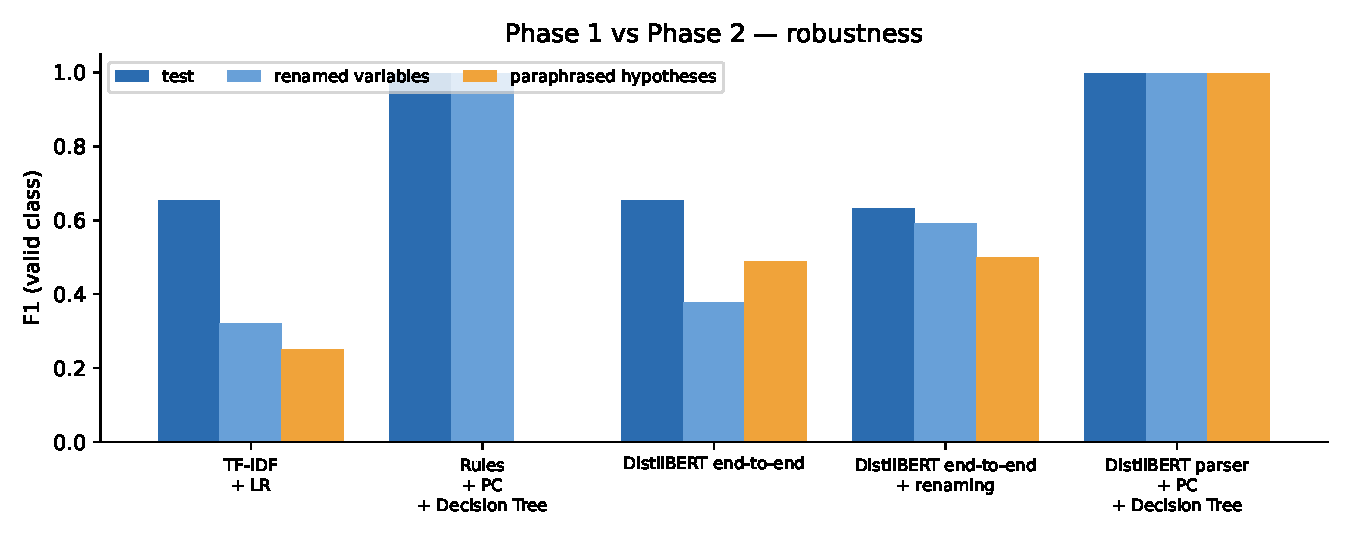
\includegraphics[width=0.95\linewidth]{figures/fig2_robustness.pdf}
\caption{Test, renamed-variable and paraphrased-hypothesis F1 for all five systems. Only 2B is high on all three.}
\label{fig:robust}
\end{figure}

\Cref{tab:main} and \cref{fig:robust} show four results:
\begin{itemize}
  \item \textbf{2A ties TF-IDF in distribution} (0.653 vs 0.655) and stays far below the symbolic reasoner. Like TF-IDF it reaches
        high recall (0.91) by calling many claims valid, at precision 0.51 (\cref{fig:conf}). Twelve thousand examples are not
        enough for DistilBERT to rediscover the PC algorithm; Jin et al.\ report the same for fine-tuned models~\cite{jin2024corr2cause}.
  \item \textbf{2A is more robust to wording than TF-IDF}: paraphrase F1 0.49 vs 0.25. Pre-training helps the language half.
  \item \textbf{Renaming augmentation removes the shortcut}: refactorization F1 rises from 0.377 to 0.592 (recall 0.46 $\rightarrow$
        0.82) for a 0.02 drop on test.
  \item \textbf{2B matches Phase~1 everywhere and fixes paraphrase}: 0.000 $\rightarrow$ 0.997. Because the parser is 100\% correct,
        by T8 2B's errors are exactly Phase~1's reasoning errors.
\end{itemize}

\begin{figure}[!htbp]
\centering
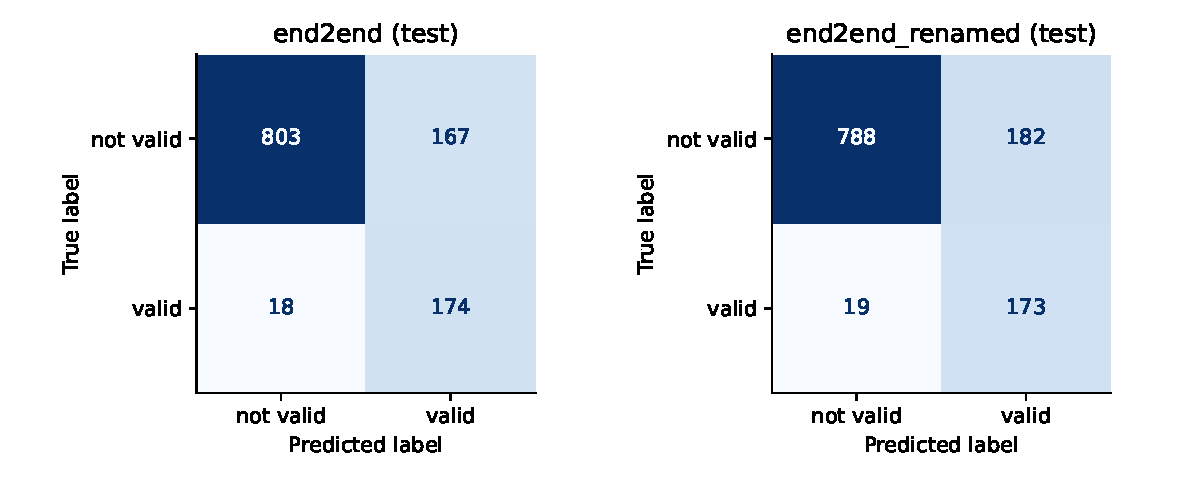
\includegraphics[width=0.8\linewidth]{figures/fig2_confusion_2a.pdf}
\caption{2A test confusion matrices. Both variants over-predict ``valid'': 167 and 182 false positives against 192 valid claims.}
\label{fig:conf}
\end{figure}

\subsection{Graph stage and intervention queries}\label{sec:graph}
The graph stage is the Phase~1 code. Only reviewed predictions enter it: claims the model calls valid with $P\ge0.5$ are
added from most to least confident, and self-loops or cycle-closing edges are rejected. Each DAG gets illustrative noisy-OR
tables in pgmpy~\cite{ankan2015}, and each of the 242 known queries ``does $\doop(X)$ change $Y$?'' is answered with the
interventional effect~\cite{pearl2009}. 2A outputs only yes/no, so to place its probabilities as edges we have to borrow the
regex reading of the test hypotheses; on paraphrased text that is impossible, so 2A has no graph there. 2B outputs triples
itself.

\begin{table}[!htbp]
\centering\small
\caption{Edge recovery (73 gold direct-cause edges on the 21 test premises) and intervention-query accuracy.}
\label{tab:graph}
\setlength{\tabcolsep}{4pt}
\begin{tabular}{@{}llcccc@{}}
\toprule
\thead{System} & \thead{Text read} & \thead{Edges} & \thead{Edge prec.} & \thead{Edge rec.} & \thead{Query acc.} \\
\midrule
2A end-to-end & test & 66/73 & 0.617 & 0.904 & 0.950 \\
\rowcolor{rowtint} 2A + renaming & test & 66/73 & 0.524 & 0.904 & 0.942 \\
Rules + PC + DT & test & 73/73 & 1.000 & 1.000 & 0.975 \\
\rowcolor{rowtint} Rules + PC + DT & paraphrase & 0/73 & 0.000 & 0.000 & 0.632 \\
\textbf{2B} & test & 73/73 & 1.000 & 1.000 & 0.975 \\
\rowcolor{rowtint} \textbf{2B} & \textbf{paraphrase} & \textbf{73/73} & \textbf{1.000} & \textbf{1.000} & \textbf{0.975} \\
\bottomrule
\end{tabular}
\end{table}

From paraphrased text Phase~1 builds empty graphs, so it can only answer ``no effect'' (0.632, the share of ``no'' queries).
2B builds the same graphs from paraphrased text as from the original wording. The six missed queries are the Phase~1 ones: chains
through an edge whose direction the correlations cannot identify.

\begin{figure}[!htbp]
\centering
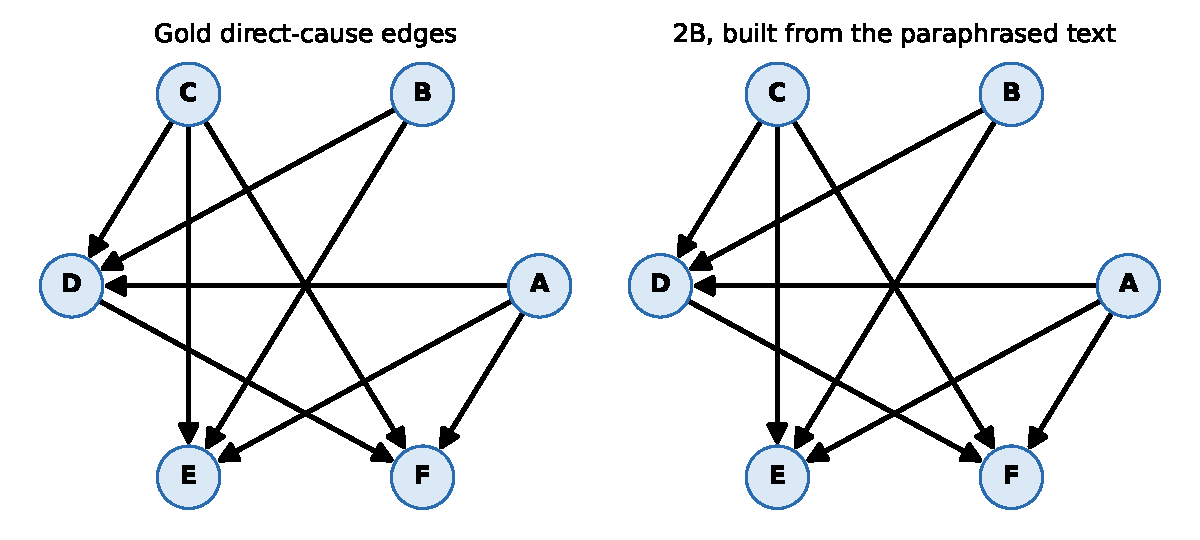
\includegraphics[width=0.75\linewidth]{figures/fig2_dag_paraphrase.pdf}
\caption{Test premise 17 (6 variables). Left: gold direct-cause edges. Right: the DAG 2B builds from the \emph{paraphrased}
hypotheses (``A directly affects B.'', ``A influences B through some mediator(s).'', \dots). They are identical.}
\label{fig:dag}
\end{figure}

\begin{table}[!htbp]
\centering\small
\caption{Documented intervention queries on the DAG of \cref{fig:dag}, built by 2B from paraphrased text.
Effect $=P(Y{=}1\mid\doop(X{=}1))-P(Y{=}1\mid\doop(X{=}0))$; ``yes'' if above 0.01.}
\label{tab:queries}
\begin{tabular}{@{}lccc@{}}
\toprule
\thead{Query} & \thead{Gold} & \thead{Effect} & \thead{Answer} \\
\midrule
does $\doop(A)$ change $F$? & yes & 0.612 & yes \\
\rowcolor{rowtint} does $\doop(B)$ change $F$? & yes & 0.328 & yes \\
does $\doop(C)$ change $D$? & yes & 0.545 & yes \\
\rowcolor{rowtint} does $\doop(D)$ change $F$? & yes & 0.545 & yes \\
does $\doop(D)$ change $A$? & no & 0.000 & no \\
\rowcolor{rowtint} does $\doop(F)$ change $C$? & no & 0.000 & no \\
\bottomrule
\end{tabular}
\end{table}

\subsection{Ablation studies}\label{sec:ablation}
Each row of \cref{tab:ablation} changes one part of a system and keeps everything else fixed.

\begin{table}[!htbp]
\centering\small
\caption{Ablations. ``Before'' and ``after'' are F1 of the valid class on the stated set.}
\label{tab:ablation}
\begin{tabularx}{\linewidth}{@{}>{\raggedright}X>{\raggedright}p{3.0cm}lcc@{}}
\toprule
\thead{What changes} & \thead{Change} & \thead{Set} & \thead{Before} & \thead{After} \\
\midrule
renaming augmentation (2A) & off $\rightarrow$ on & refactorization & 0.377 & 0.592 \\
\rowcolor{rowtint} language layer (reasoning fixed: PC + tree) & regex $\rightarrow$ DistilBERT & paraphrase & 0.000 & 0.997 \\
reasoning layer (DistilBERT in both) & none $\rightarrow$ PC + tree & test & 0.653 & 0.997 \\
\rowcolor{rowtint} text-only model & TF-IDF $\rightarrow$ DistilBERT & paraphrase & 0.250 & 0.489 \\
\bottomrule
\end{tabularx}
\end{table}

The ablations separate the two halves of the problem. Swapping the \emph{language} model helps on new wordings
(rows 2 and 4). Adding the \emph{reasoning} layer is what makes the answers correct (row 3: +0.34 F1). The Phase~1 feature
ablation (support and PC-graph features carry the signal) still holds, since 2B uses the same features.

% =====================================================================
\section{Error Analysis and Limitations}\label{sec:errors}

\begin{table}[!htbp]
\centering\small
\caption{2A test error rate by relation type and by number of variables.}
\label{tab:errors}
\begin{tabular}{@{}lcc@{\hspace{2em}}lcc@{}}
\toprule
\thead{Relation} & \thead{2A} & \thead{2A + ren.} & \thead{Variables} & \thead{2A} & \thead{2A + ren.} \\
\midrule
collider   & 0.492 & 0.435 & 2 & 0.167 & 0.167 \\
\rowcolor{rowtint} confounder & 0.052 & 0.067 & 3 & 0.167 & 0.271 \\
direct     & 0.124 & 0.173 & 4 & 0.250 & 0.236 \\
\rowcolor{rowtint} indirect   & 0.082 & 0.095 & 5 & 0.210 & 0.245 \\
           &       &       & 6 & 0.096 & 0.084 \\
\bottomrule
\end{tabular}
\end{table}

\begin{itemize}
  \item \textbf{2A fails at reasoning, mostly on colliders.} Almost half of 2A's collider claims are wrong (\cref{tab:errors}). A
        collider is identified by an \emph{independence} fact plus two correlations, a combination spread across the premise.
        This is the step the PC algorithm does with one rule (Phase~1, T2) and the hardest for a model learning from examples.
        Of 20 randomly sampled wrong predictions of 2A + renaming (201 in total), 18 come from 5- and 6-variable premises.
  \item \textbf{2B's errors are Phase~1's errors.} 2B is wrong on 0 of 1{,}076 dev, 1 of 1{,}162 test, 2 of 2{,}246 refactorization
        and 2 of 2{,}246 paraphrase rows. The two paraphrase errors (``Some variable(s) cause(s) both E and F.'') are parsed
        correctly as confounder(E, F); the tree rejects them through the same confounder quirk of the dataset generator that
        causes Phase~1's single test error. As T8 predicts, the language layer adds no new errors.
  \item \textbf{The paraphrase test is narrow.} It has only four wordings. We added unseen-verb validation and demo sentences, but
        free text (news, PubMed) would need a richer grammar or real annotated sentences. The grammar was written knowing the test
        vocabulary existed, so we banned those words rather than imitating them.
  \item \textbf{Two variables per claim.} The parser assumes a hypothesis names exactly two variables. Claims about three or more
        (``A affects B only through C'') are rejected, not misread.
  \item \textbf{Small 2A run.} 12k training pairs and batch 8 are laptop limits. A larger run may narrow the gap to TF-IDF, but the
        Corr2Cause authors' larger fine-tuned models also failed under perturbation~\cite{jin2024corr2cause}, so we do not expect it
        to close the gap to the symbolic reasoner.
  \item \textbf{Illustrative probabilities.} As in Phase~1, the noisy-OR tables are assumptions; the effects show the mechanism, not
        real effect sizes.
\end{itemize}

% =====================================================================
\section{Reproducibility and Code Quality}\label{sec:repro}

Phase~2 adds four modules and one script; no Phase~1 module was changed.

\begin{examplebox}
\footnotesize
\begin{tabularx}{\linewidth}{@{}>{\ttfamily}l@{\hspace{1.2em}}>{\raggedright\arraybackslash}X@{}}
src/causal\_nlp/dl\_common.py         & DistilBERT training loop (plain PyTorch), prediction, save / load \\
src/causal\_nlp/dl\_end2end.py        & 2A: training sample, renaming augmentation, end-to-end classifier \\
src/causal\_nlp/paraphrase\_grammar.py & 2B: grammar that writes the parser's training sentences \\
src/causal\_nlp/dl\_parser.py         & 2B: labels, leak check, held-out verbs, \texttt{DistilBertParser} (drop-in for the regex) \\
tools/train\_phase2.py               & trains the three models into \texttt{models/} (not in git) \\
notebooks/02\_phase2\_dl\_pipeline.ipynb & executed Phase~2 deliverable; trains any missing model first \\
tests/test\_phase2.py                & 18 unit tests (32 with Phase~1) \\
\end{tabularx}
\end{examplebox}

\begin{itemize}
  \item \textbf{Readable training loop.} \code{train\_classifier} is a hand-written PyTorch loop~\cite{paszke2019} (tokenise $\rightarrow$
        batch $\rightarrow$ forward $\rightarrow$ weighted loss $\rightarrow$ backward $\rightarrow$ AdamW step) rather than a library trainer, so
        every step can be explained. Models and tokenizers come from Hugging Face Transformers~\cite{wolf2020}.
  \item \textbf{Drop-in layer.} \code{DistilBertParser} has the same call signature as the regex parser, so
        \code{build\_feature\_table(inputs, hypothesis\_parser=parser)} and \code{graph\_stage} run unchanged.
  \item \textbf{Tested.} All 32 tests pass (\code{pytest -q}, about 7\,s, no training). The Phase~2 tests check, for example, that renaming
        keeps every correlation fact, that no training template uses a test phrase, that held-out verbs never appear in training, and
        that generated labels agree with the Phase~1 regex parser.
  \item \textbf{Deterministic.} Seed 42, pinned versions (\code{torch 2.15}, \code{transformers 5.22}). Training: about 1 hour in total on an
        Apple M3 Pro GPU. On a bigger GPU, train 2A on more data with\\
        \code{END2END\_ROWS=40000 END2END\_BATCH=16 python tools/train\_phase2.py end2end}.
\end{itemize}

% =====================================================================
\section{Conclusion}\label{sec:conclusion}
Phase~2 asked where a transformer helps a causal-inference pipeline. Given the whole job (2A), DistilBERT learns the wording but
not the reasoning: it ties a TF-IDF baseline and needs augmentation to stop exploiting variable names. Given only the language job
(2B), it reads every paraphrased and unseen-verb hypothesis correctly, and the unchanged symbolic layers turn those readings into
the same near-perfect answers, DAGs and intervention results Phase~1 produced on the original wording. Language models are good
at language and not, on their own, at causal inference~\cite{kiciman2023}; the hybrid uses each part for what it does well.

% =====================================================================
\section{Team Contributions}
\begin{table}[!htbp]
\centering\small
\begin{tabularx}{\linewidth}{@{}lX@{}}
\toprule
\thead{Member} & \thead{Phase 2 responsibility} \\
\midrule
\MemberA & Phase~2 notebook: evaluation, graph stage, ablations, final comparison; report (\cref{sec:results,sec:graph,sec:ablation}) \\
\rowcolor{rowtint} \MemberB & DistilBERT training loop, dependencies, hyper-parameters and regularization (\cref{sec:theory,tab:hparams,tab:reg}) \\
\MemberC & 2A end-to-end classifier, training sample and renaming augmentation (\cref{sec:arch2a,sec:data2a}) \\
\rowcolor{rowtint} \MemberD & Training script and Phase~2 unit tests (\cref{sec:repro}) \\
\MemberE & 2B language layer: parser grammar, DistilBERT parser, leak check and held-out-verb validation (\cref{sec:arch2b,sec:data2b}) \\
\bottomrule
\end{tabularx}
\end{table}

% =====================================================================
\begingroup
\small
\renewcommand{\refname}{References}
\begin{thebibliography}{99}\setlength{\itemsep}{2pt}
\bibitem{jin2024corr2cause} Z.~Jin, J.~Liu, Z.~Lyu, S.~Poff, M.~Sachan, R.~Mihalcea, M.~Diab, and B.~Sch\"olkopf, ``Can large language models infer causation from correlation?'' in \emph{Proc.\ ICLR}, 2024.
\bibitem{corr2causecorrected} Corr2Cause corrected labels, Hugging Face dataset \texttt{zluke/corr2cause-corrected}, \url{https://huggingface.co/datasets/zluke/corr2cause-corrected}.
\bibitem{pearl1988} J.~Pearl, \emph{Probabilistic Reasoning in Intelligent Systems: Networks of Plausible Inference}. Morgan Kaufmann, 1988.
\bibitem{pearl2009} J.~Pearl, \emph{Causality: Models, Reasoning, and Inference}, 2nd~ed. Cambridge University Press, 2009.
\bibitem{spirtes2000} P.~Spirtes, C.~Glymour, and R.~Scheines, \emph{Causation, Prediction, and Search}, 2nd~ed. MIT Press, 2000.
\bibitem{verma1990} T.~Verma and J.~Pearl, ``Equivalence and synthesis of causal models,'' in \emph{Proc.\ UAI}, 1990, pp.~255--270.
\bibitem{meek1995} C.~Meek, ``Causal inference and causal explanation with background knowledge,'' in \emph{Proc.\ UAI}, 1995, pp.~403--410.
\bibitem{ankan2015} A.~Ankan and A.~Panda, ``pgmpy: Probabilistic graphical models using Python,'' in \emph{Proc.\ SciPy}, 2015, pp.~6--11.
\bibitem{khoo2000} C.~S.~G.~Khoo, S.~Chan, and Y.~Niu, ``Extracting causal knowledge from a medical database using graphical patterns,'' in \emph{Proc.\ ACL}, 2000, pp.~336--343.
\bibitem{girju2003} R.~Girju, ``Automatic detection of causal relations for question answering,'' in \emph{Proc.\ ACL Workshop on Multilingual Summarization and Question Answering}, 2003, pp.~76--83.
\bibitem{vaswani2017} A.~Vaswani, N.~Shazeer, N.~Parmar, J.~Uszkoreit, L.~Jones, A.~N.~Gomez, {\L}.~Kaiser, and I.~Polosukhin, ``Attention is all you need,'' in \emph{Proc.\ NeurIPS}, 2017, pp.~5998--6008.
\bibitem{devlin2019} J.~Devlin, M.-W.~Chang, K.~Lee, and K.~Toutanova, ``BERT: Pre-training of deep bidirectional transformers for language understanding,'' in \emph{Proc.\ NAACL-HLT}, 2019, pp.~4171--4186.
\bibitem{sanh2019} V.~Sanh, L.~Debut, J.~Chaumond, and T.~Wolf, ``DistilBERT, a distilled version of BERT: smaller, faster, cheaper and lighter,'' arXiv:1910.01108, 2019.
\bibitem{hinton2015} G.~Hinton, O.~Vinyals, and J.~Dean, ``Distilling the knowledge in a neural network,'' arXiv:1503.02531, 2015.
\bibitem{wolf2020} T.~Wolf \emph{et al.}, ``Transformers: State-of-the-art natural language processing,'' in \emph{Proc.\ EMNLP: System Demonstrations}, 2020, pp.~38--45.
\bibitem{paszke2019} A.~Paszke \emph{et al.}, ``PyTorch: An imperative style, high-performance deep learning library,'' in \emph{Proc.\ NeurIPS}, 2019, pp.~8024--8035.
\bibitem{loshchilov2019} I.~Loshchilov and F.~Hutter, ``Decoupled weight decay regularization,'' in \emph{Proc.\ ICLR}, 2019.
\bibitem{howard2018} J.~Howard and S.~Ruder, ``Universal language model fine-tuning for text classification,'' in \emph{Proc.\ ACL}, 2018, pp.~328--339.
\bibitem{sun2019} C.~Sun, X.~Qiu, Y.~Xu, and X.~Huang, ``How to fine-tune BERT for text classification?'' in \emph{Proc.\ China National Conference on Chinese Computational Linguistics (CCL)}, 2019, pp.~194--206.
\bibitem{mosbach2021} M.~Mosbach, M.~Andriushchenko, and D.~Klakow, ``On the stability of fine-tuning BERT: Misconceptions, explanations, and strong baselines,'' in \emph{Proc.\ ICLR}, 2021.
\bibitem{srivastava2014} N.~Srivastava, G.~Hinton, A.~Krizhevsky, I.~Sutskever, and R.~Salakhutdinov, ``Dropout: A simple way to prevent neural networks from overfitting,'' \emph{Journal of Machine Learning Research}, vol.~15, pp.~1929--1958, 2014.
\bibitem{prechelt1998} L.~Prechelt, ``Early stopping --- but when?'' in \emph{Neural Networks: Tricks of the Trade}, Springer, 1998, pp.~55--69.
\bibitem{pascanu2013} R.~Pascanu, T.~Mikolov, and Y.~Bengio, ``On the difficulty of training recurrent neural networks,'' in \emph{Proc.\ ICML}, 2013, pp.~1310--1318.
\bibitem{he2009} H.~He and E.~A.~Garcia, ``Learning from imbalanced data,'' \emph{IEEE Transactions on Knowledge and Data Engineering}, vol.~21, no.~9, pp.~1263--1284, 2009.
\bibitem{gururangan2018} S.~Gururangan, S.~Swayamdipta, O.~Levy, R.~Schwartz, S.~Bowman, and N.~A.~Smith, ``Annotation artifacts in natural language inference data,'' in \emph{Proc.\ NAACL-HLT}, 2018, pp.~107--112.
\bibitem{mccoy2019} R.~T.~McCoy, E.~Pavlick, and T.~Linzen, ``Right for the wrong reasons: Diagnosing syntactic heuristics in natural language inference,'' in \emph{Proc.\ ACL}, 2019, pp.~3428--3448.
\bibitem{geirhos2020} R.~Geirhos, J.-H.~Jacobsen, C.~Michaelis, R.~Zemel, W.~Brendel, M.~Bethge, and F.~A.~Wichmann, ``Shortcut learning in deep neural networks,'' \emph{Nature Machine Intelligence}, vol.~2, pp.~665--673, 2020.
\bibitem{ribeiro2020} M.~T.~Ribeiro, T.~Wu, C.~Guestrin, and S.~Singh, ``Beyond accuracy: Behavioral testing of NLP models with CheckList,'' in \emph{Proc.\ ACL}, 2020, pp.~4902--4912.
\bibitem{kaushik2020} D.~Kaushik, E.~Hovy, and Z.~C.~Lipton, ``Learning the difference that makes a difference with counterfactually-augmented data,'' in \emph{Proc.\ ICLR}, 2020.
\bibitem{wei2019} J.~Wei and K.~Zou, ``EDA: Easy data augmentation techniques for boosting performance on text classification tasks,'' in \emph{Proc.\ EMNLP-IJCNLP}, 2019, pp.~6382--6388.
\bibitem{wang2015} Y.~Wang, J.~Berant, and P.~Liang, ``Building a semantic parser overnight,'' in \emph{Proc.\ ACL-IJCNLP}, 2015, pp.~1332--1342.
\bibitem{jia2016} R.~Jia and P.~Liang, ``Data recombination for neural semantic parsing,'' in \emph{Proc.\ ACL}, 2016, pp.~12--22.
\bibitem{lake2018} B.~Lake and M.~Baroni, ``Generalization without systematicity: On the compositional skills of sequence-to-sequence recurrent networks,'' in \emph{Proc.\ ICML}, 2018, pp.~2873--2882.
\bibitem{garcez2023} A.~d'Avila Garcez and L.~C.~Lamb, ``Neurosymbolic AI: The 3rd wave,'' \emph{Artificial Intelligence Review}, vol.~56, pp.~12387--12406, 2023.
\bibitem{mao2019} J.~Mao, C.~Gan, P.~Kohli, J.~B.~Tenenbaum, and J.~Wu, ``The neuro-symbolic concept learner: Interpreting scenes, words, and sentences from natural supervision,'' in \emph{Proc.\ ICLR}, 2019.
\bibitem{kiciman2023} E.~K{\i}c{\i}man, R.~Ness, A.~Sharma, and C.~Tan, ``Causal reasoning and large language models: Opening a new frontier for causality,'' arXiv:2305.00050, 2023.
\end{thebibliography}
\endgroup

\end{document}
